\documentclass{beamer}
\usepackage[brazil]{babel}
\usepackage[utf8]{inputenc}
\usepackage{times}
\usepackage[T1]{fontenc}
%\usepackage{subfigure}
%\usepackage{wrapfig}
\usepackage{float}
\usepackage{ctable}
\usepackage{colortbl}

\usepackage{pgfpages}

\mode<presentation>
{
  \usetheme{Singapore}
  \usecolortheme{rose}
  %\usefonttheme[onlylarge]{structurebold}
  %\setbeamerfont*{frametitle}{size=\normalsize,series=\bfseries}
  % or ...
  \setbeamercovered{transparent}
  % or whatever (possibly just delete it)
  \setbeamertemplate{navigation symbols}{}
  \setbeamertemplate{note page}[plain]
  %\logo{\includegraphics[width=1.2 cm]{figuras/logo_ufes}}
  \setbeamertemplate{footline}{\hfill\scriptsize{\vspace*{5pt}\color{gray}{\insertframenumber}\hspace*{5pt}}} 
  %\setbeamertemplate{footline}{%
  %\leavevmode%
  %\hbox{%
  %\begin{beamercolorbox}[wd=.5\paperwidth,ht=2.25ex,dp=1ex,right]{author in
  %    head/foot}%
  %    \usebeamerfont{author in head/foot}\insertshortauthor \hspace{.5cm}
  %    (\insertshortinstitute) \hspace{.5cm}
  %\end{beamercolorbox}%

  %\begin{beamercolorbox}[wd=.5\paperwidth,ht=2.25ex,dp=1ex,left]{title in
  %    head/foot}%
  %    \usebeamerfont{title in head/foot} \hspace{.5cm}\insertshorttitle
  %\end{beamercolorbox}}%
  %\vskip0pt%
  %}
}

% Define o tema da apresentacao (soh fica guardado nas informacoes do pdf)
\subject{Detecção de drift em sensores}
% Delete this, if you do not want the table of contents to pop up at
% the beginning of each subsection:
% \AtBeginSubsection[]
% {
%   \begin{frame}<beamer>{Sumário}
%     \tableofcontents[currentsection,currentsubsection]
%   \end{frame}
% }
 \AtBeginSection[]
 {
   \begin{frame}<beamer>{Sumário}
     \tableofcontents[currentsection]
   \end{frame}
 }
%\setbeameroption{show notes}
%\setbeameroption{show notes on second screen=right}
%============================================================================================

\title
[Algoritmos para a Detecção de \textit{Drifting} em Sensores de Poços de Petróleo]
{Algoritmos para a Detecção de \textit{Drifting} em Sensores de Poços de Petróleo}

\author[Boechat A.A.]
{ 
    André Ambrósio Boechat
}
\institute[UFSC]{Departamento de Automação e Sistemas\\Universidade Federal de Santa
Catarina}

%Programa de Pós-Graduação em Eng. de Automação e Sistemas\\Universidade Federal
%de Santa Catarina
%}

% Se comentar a linha abaixo, ira aparecer a data quando foi compilada a apresentacao
\date{Florianópolis, Agosto de 2012}

\setbeamercolor{postit}{fg=black,bg=block body.fg!75!black!10!bg}
% =========================================================================================
\begin{document}

\begin{frame}
    \titlepage
    \thispagestyle{empty}

    \note{
    \begin{itemize}
        \item trabalho de mestrado sob orientação do prof. Ubirajara
    \end{itemize}}
\end{frame}


\begin{frame}{Sumário}
    \tableofcontents[]
\end{frame}

\section{Introdução}
\subsection{}

\begin{frame}{Sensores na Indústria Petrolífera}
    \begin{itemize}
        \item Desempenham importantes papéis
            \begin{itemize}
                \item ações de controle
                \item otimização da produção
                \item monitoramento do poço
                \item monitoramento do desempenho de equipamentos
                \item tomada de decisões
            \end{itemize}
        \item Crescimento do número de sensores
        \item Localizados em pontos críticos
            \begin{itemize}
                \item difícil acesso
                \item ambientes inóspitos
            \end{itemize}
    \end{itemize}

    \begin{block}{Problema}
        As informações fornecidas pelos sensores são \alert{confiáveis}?
    \end{block}

    \note{
    \begin{itemize}
        \item sensores são como os sentidos humanos para a indústria
        \item monitoramento do poço: mudanças nas características
        \item crescimento do número de sensores: queda dos preços, espalhando por todos os
            lugares, como nos celulares (acelerômetros, sensor de luz)
        \item ambientes inóspitos, degradantes: alta temperatura, pressão, etc.
    \end{itemize}
    }
\end{frame}

\begin{frame}{\textit{Drift} em Sensores}
    Desvio lento e contínuo das medições ao longo do tempo

    \begin{itemize}
        \item Um dos problemas mais comuns em sensores
        \item Difícil detecção
            \begin{itemize}
                \item comparação com sinais de outros sensores
                \item detectável quando os desvios são grosseiros
            \end{itemize}
    \end{itemize}

    \begin{beamercolorbox}[sep=5pt]{postit}
        ``Leituras realizadas por um sensor instável ou com desvios excessivos
        normalmente são mais problemáticos a um operador que a falha completa do
        sensor.''\\ \footnotesize(Joseph Eck et al., 1999)
    \end{beamercolorbox}

    \begin{figure}[!htb]
        \centering
        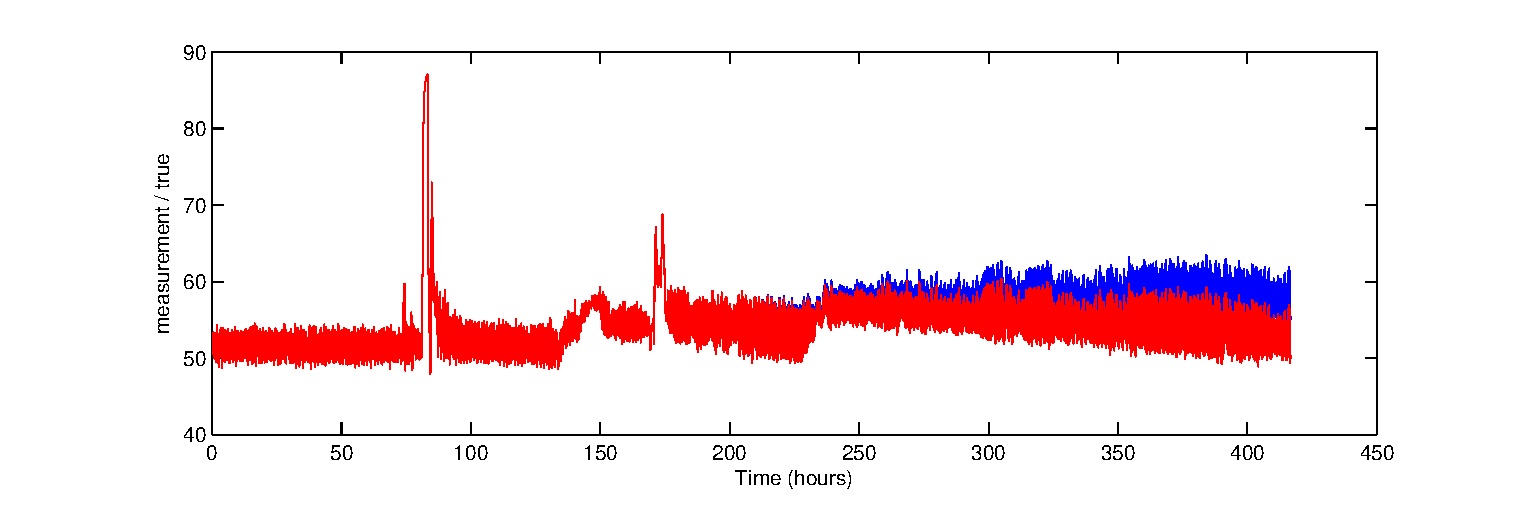
\includegraphics[trim=0pt 0pt 0cm 15pt,clip=true,width=\textwidth]{figuras/drift.eps}
    \end{figure}

    \note{
    Um dos principais problemas que ocorrem com sensores e é o foco da dissertação.

    \begin{itemize}
        \item Dificuldade de detecção manual: depende da comparação com os sinais de
            outros sensores, das ações dos operadores, além de ser perceptível apenas
            quando os desvios são grosseiros.
        \item Frase sobre falha de sensor: tomar decisões baseadas em falsas informações
            pode ser mais perigoso que decisões baseadas na falta da informação.
    \end{itemize}
    }
\end{frame}

\begin{frame}{Proposta do Trabalho}

    \begin{itemize}
        \item Estratégia de manutenção \alert{CBM}
        \item Modelos empíricos baseados em \alert{histórico}
    \end{itemize}
    
\end{frame}

\section{Estrutura de Sistemas de Manutenção CBM}
\subsection{}

\begin{frame}{Estratégias de Manutenção}

        CBM (\textit{Condition Based Maintenance})\\
            Manuntenção baseada na condição de funcionamento

    \begin{block}{Estratégia tradicional}
        \begin{itemize}
            \item Manutenção periódica
            \item Manutenção reativa
        \end{itemize}
    \end{block}

    \begin{block}{CBM}
        \begin{itemize}
            \item Monitoramento da condição de funcionamento
            \item Manutenção apenas quando realmente necessário
            \item Agendamento dinâmico de manutenções
            \item Planejamento de acordo com as condições
            \item Redução de manutenções reativas (menos surpresas)
        \end{itemize}
    \end{block}
    
\end{frame}


\begin{frame}{Implementação de Sistemas de Manutenção CBM}

    \begin{block}{Dificuldades}
        \begin{itemize}
            \item Grande volume de dados coletados
                \pause
            \item Dados provindos de sistemas geograficamente dispersos
                \pause
            \item Integração dos dados
                \pause
            \item Escalabilidade
                \pause
            \item Disponibilidade de conhecimentos especialistas
                \pause
        \end{itemize}
    \end{block}

    \begin{block}{Benefícios de uma arquitetura modular e padronizada}
        \begin{itemize}
            \item Facilidade de atualização de componentes
                \pause
            \item Facilidade para se tornar um fornecedor de soluções
                \pause
            \item Redução de preços e custos
        \end{itemize}
        
    \end{block}

    \note{
    \begin{itemize}
        \item volume de dados: coletados de vários partes de vários processos
        \item integração: em muitos casos, informações úteis surgem apenas a integração
            dos dados de diferentes fontes e tipos
        \item escalabilidade: com o tempo pode surgir a necessidade de adicionar novas fontes
            de dados
        \item conhecimentos especialistas: necessário para extrair informações úteis para
            manutenção
        \item atualização de componentes: mudanças em componentes não necessitariam de
            mudanças em outras partes do sistema
        \item fornecedor: não é necessário conhecer todo o sistema, facilidade de
            integrar uma solução ao sistema, possibilidade de se focar em problemas
            menores (detecção de estado estacionário, por exemplo)
        \item redução de custos: como o sistema torna-se dividido em partes independentes,
            concorrência entre fornecedores 
    \end{itemize}}
    
\end{frame}

\begin{frame}{OSA-CBM}
    
    \centering
    Resultado de um parceria entre indústrias, fabricantes, universidades e a Marinha
    Norte-Americana

    \begin{figure}[!htb]
        \centering
        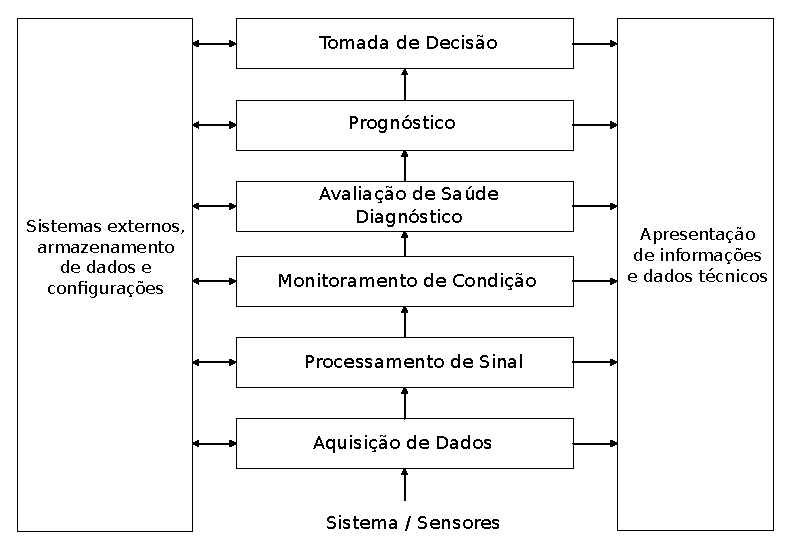
\includegraphics[width=.9\textwidth]{figuras/arte/osa_cbm_camadas.eps}
    \end{figure}

    \note{
    \begin{itemize}
        \item é uma arquitetura aberta para sistemas de manutenção na condição de operação
        \item OSA-CBM ainda faz parte de uma arquitura maior, que incorpora a manutenção
            com gerência de recursos humanos e de maquinários e as decisões de negócio
        \item processamento de sinais:
    \end{itemize}}
    
\end{frame}


\section{Sistemas de Validação de Sensores}
\subsection{}

\begin{frame}{Avaliação do Desempenho de Sensores}
    \begin{block}{Abordagem tradicional}
        \begin{itemize}
            \item calibração manual periódica
                \begin{itemize}
                    \item não se conhece a real necessidade
                    \item instrumentos são retirados de operação
                \end{itemize}
        \end{itemize}
    \end{block}

    \begin{block}{Manutenção baseada na condição (CBM)}
        \begin{itemize}
            \item monitora-se a \alert{condição} de funcionamento
            \item calibrações físicas apenas quando realmente \alert{necessário}
            \item tendem a ser menos invasivas e mais eficazes
                \vspace{6pt}
            \item redundância por \textit{hardware}
            \item redundância \alert{analítica}
                \begin{itemize}
                    \item equações fenomenológicas
                    \item modelos empíricos baseados em \alert{histórico}
                \end{itemize}
        \end{itemize}
        
    \end{block}

    \note{
    \begin{itemize}
        \item necessidade da calibração periódica: desperdício de tempo, dinheiro,
            mão-de-obra ou usa-se de forma descalibrada sem saber, mesmo que por um
            determinado período de tempo

        \item calibrações físicas no CBM: leituras podem ser ajustadas via software ou
            corrige-se as leituras conhecendo-se os erros

        \item CBM menos invasivas e mais eficazes: pelos dois motivos citados
            anteriormente sobre a calibração manual
            \vspace{15pt}
        \item redundância por hardware: necessidade de inclusão de novos sensores, espaço
            e energia limitado em um poço
        \item eqs fenomenológicas: são normalmente bem precisos, mas necessitam de grandes
            esforços de engenharia e podem ser sensíveis a mudanças ou degradações não
            previstas no sistema
    \end{itemize}}
    
\end{frame}

\begin{frame}{Abordagem por Modelos Baseados em Histórico}
    
    \begin{figure}[!htb]
        \centering\hspace*{-20pt}
        \includegraphics[width=1.1\textwidth]{figuras/data_driven_fdd.eps}
    \end{figure}
    
    \note{
    \begin{itemize}
        \item dados de treinamento: precisam estar livre de falhas e representar as
            condições de funcionamento esperadas para o futuro
        \item predição: imitar as leituras de sensores a partir de sensores
            correlacionados
        % \item na verdade, este diagrama poderia representar também a redundância por
        %     equações fenomenológicas
    \end{itemize}}
\end{frame}



% \begin{frame}{Benefícios de Sistemas de Manutenção CBM}
% 
%     \begin{itemize}
%         \item Manutenções agendadas \alert{dinamicamente}
%             \pause
%         \item Redução do tempo de \alert{inatividade}
%             \pause
%         \item Ganho de \alert{desempenho} dos sistemas
%             \pause
%         \item Prolongamento da \alert{vida útil} de equipamentos
%             \pause
%         \item Melhor utilização de \alert{recursos humanos} limitados
%         \item Redução de \alert{custos}\\
%             $\vdots$
%             \pause
%         \item Produção gradualmente mais \alert{efetiva}
%     \end{itemize}
% 
%     \note{
%         Para entender a necessidade de se pensar com cuidado na estrutura desses sistemas,
%         é necessário primeiro apontar os potenciais benefícios dos sistemas e depois
%         discutir sobre as dificuldades de se implementar
%     \begin{itemize}
%         \item agendamento dinâmico: de acordo com a real necessidade
%         \item tempo de inatividade: paradas desnecessárias não acontecem, falhas são
%             previstas e as ações são planejadas
%         \item desempenho dos sistemas: tendem a funcionar da melhor forma possível por
%             mais tempo
%         \item prolongamento da vida útil: equipamentos funcionam da melhor maneira
%             possível por maior tempo
%         \item recursos humanos: consequência do melhor planejamento
%     \end{itemize}}
% \end{frame}





\begin{frame}{Validação de Sensores e a OSA-CBM}

    \begin{figure}[!htb]
        \centering
        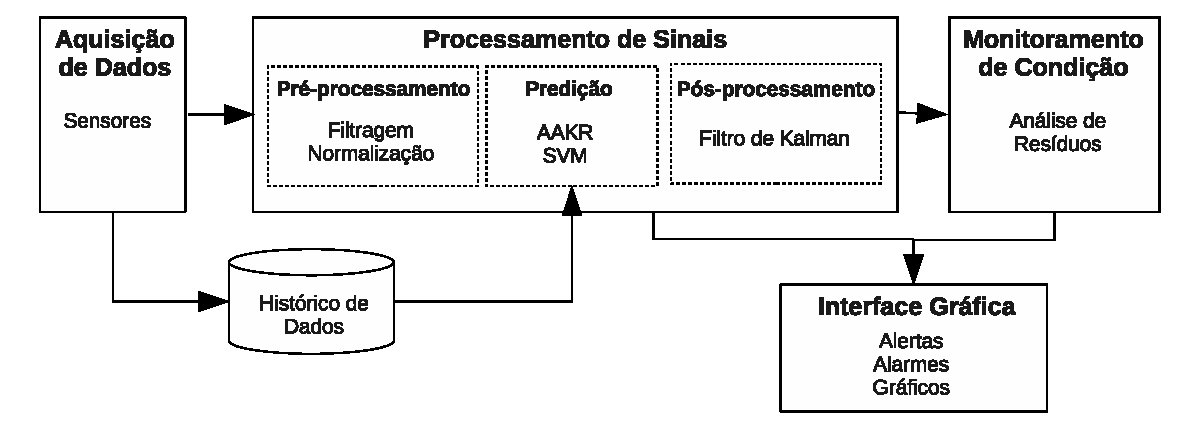
\includegraphics[width=\textwidth]{figuras/osa_cbm_drift.eps}\\
        \includegraphics[width=.8\textwidth]{figuras/data_driven_fdd.eps}
    \end{figure}

    \note{
    \begin{itemize}
        \item explicar bem o que significa a limpeza dos dados
        \item filtragem: remoção de dados espúrios (outliers) e ruídos dos dados de
            treinamento, apenas informações verdadeiras são absorvidas pelos modelos
        \item dizer por cima a parte de predição, como feito no diagrama de um sistema de
            validação, imitação das leituras de um sensor a partir de medidas de sensores
            correlacionados
    \end{itemize}}
    
\end{frame}

\begin{frame}{Predição das Leituras dos Sensores}

    \begin{block}{AAKR - Regressão por kernel auto-associativa}
        \begin{itemize}
            \item Estrutura auto-associativa
            %\item não há um processo real de treinamento
            \item Predições baseadas na similaridade entre as entradas e os vetores de
                memória
            \item Dois parâmetros de sintonia: número de vetores ($n_m$) e largura de
                banda ($h$)
        \end{itemize}
    \end{block}

    \begin{block}{SVM - \textit{Support Vector Machines}}
        \begin{itemize}
            \item Estrutura inferencial
            \item Processo de treinamento constrói uma $f(\mathbf{r}) \approx y$ 
            \item Três parâmetros de sintonia: $\varepsilon$, $C$ e $\gamma$
        \end{itemize}
        
    \end{block}

    \note{
        AAKR
    \begin{itemize}
        \item auto-associativa: as saídas imitam as próprias entradas
        \item número de vetores: número alto pode garantir uma melhor cobertura dos pontos
            de operação, mas torna as predições computacionalmente mais custosas; baixo
            número, podem faltar informações
        \item largura de banda: controla a suavidade das predições
    \end{itemize}
        SVM
    \begin{itemize}
        \item inferencial: as leituras de um sensor são estimadas a partir de outros
            sensores apenas, as próprias leituras são desprezadas
    \end{itemize}}
    
\end{frame}

\begin{frame}{Geração de Resíduos}

    \begin{itemize}
        \item Diferenças entre as leituras dos sensores e as predições dos modelos
    \end{itemize}
    
    \begin{figure}[!htb]
        \centering Sistema 1
        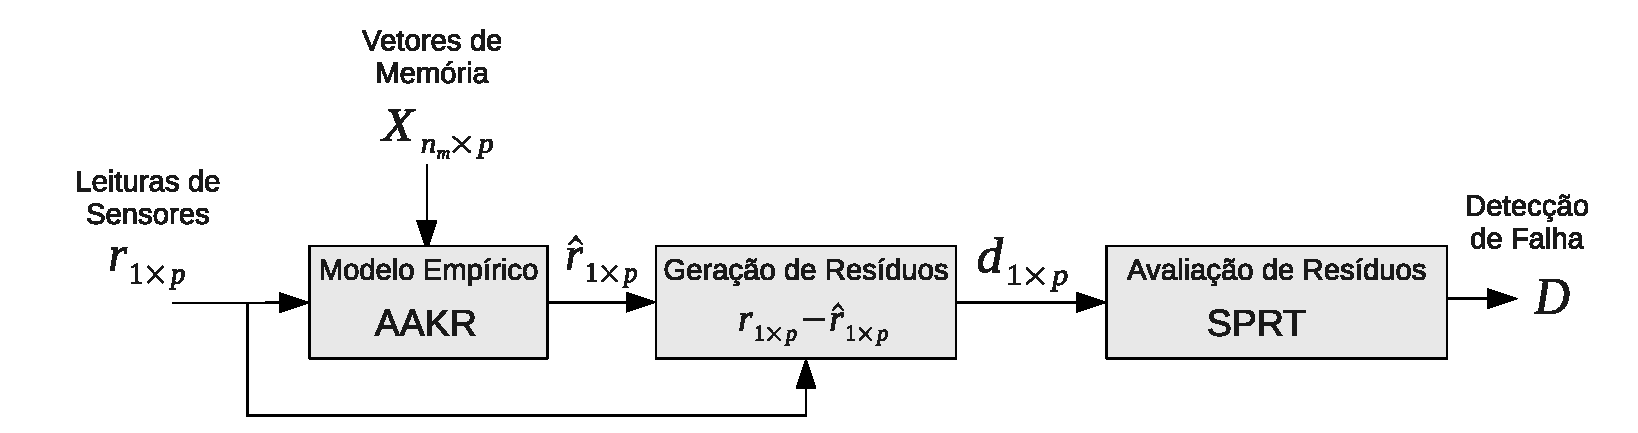
\includegraphics[width=.8\textwidth]{figuras/aakr_sprt.eps}
    \end{figure}
    
    \begin{figure}[!htb]
        \centering Sistema 2
        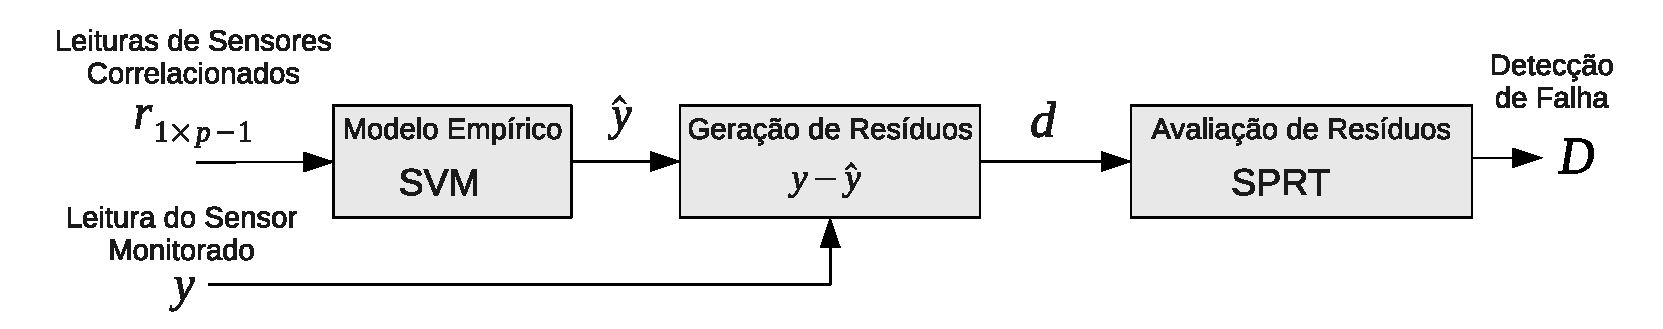
\includegraphics[width=.8\textwidth]{figuras/svm_sprt.eps}
    \end{figure}
\end{frame}

\begin{frame}{Monitoramento da Condição\\SPRT}
    \textit{Sequential Probability Ratio Test}
    
    \begin{itemize}
        \item Algoritmo para detecção de propriedades estatísticas
        \item Testes para verificar qual a distruição de probabilidade
            \begin{itemize}
                \item modo normal $H_0$: distribuição Normal, média zero e variância
                    semelhante a do ruído
                \item modo degradado $H_1$: distribuição Normal, média diferente de zero e
                    variância semelhante a do ruído
            \end{itemize}
    \end{itemize}
    $$
    \Lambda^{(i)} = \ln \frac{P(d^{(i)} | H_1)}{P(d^{(i)} | H_0)}
    \label{eq:loglikelihood}
    $$
    \begin{itemize}
        \item Parâmetro de sintonia $M$, diferença tolerável na média
    \end{itemize}

\end{frame}

% \begin{frame}{Monitoramento da Condição}
% 
%     \begin{itemize}
%         \item Resíduos: diferença entre as predições
%         \item Normalidade: média zero e variância semelhante a do ruído no sensor
%     \end{itemize}
% 
%     \begin{block}{Detecção de falhas e desvios (\textit{drift})}
%         Detecção de mudanças nas propriedades estatísticas dos resíduos
%     \end{block}
% 
%     \begin{itemize}
%         \item Algoritmo de detecção: SPRT (\textit{Sequential Probability Ratio Test}),
%             parâmetro $M$
%     \end{itemize}
% 
%     \begin{figure}[!htb]
%         \centering
%         \includegraphics[width=\textwidth]{figuras/residual_ex.eps}
%     \end{figure}
% 
%     \note{
%     \begin{itemize}
%         \item A detecção consiste em detectar um estado diferente da normalidade
%         \item $M$: praticamente a amplitude do desvio, limiar ou threshold
%         \item o SPRT é usado para detecção de mudanças em propriedades estatísticas, neste
%             caso, a média
%     \end{itemize}}
%     
% \end{frame}

\begin{frame}{Filtro de Kalman}

    \begin{beamercolorbox}[sep=5pt]{postit}
        Estima continuamente os desvios presentes no sensor
    \end{beamercolorbox}

    \begin{itemize}
        \item Considerações:
            \begin{itemize}
                \item suavidade
                \item crescimento lento
                \item linear ou exponencial
                \item descorrelacionado com desvios de outros sensores
            \end{itemize}
    \end{itemize}

    Atualização das estimativas
    $$
    {d}^{(k)} = {d}^{(k-1)} + {v}^{(k)}, \quad {v}^{(k)} \sim \mathcal{N} ({0}, \sigma_v)
    $$

    Observação
    $$
    {z} = {d}^{(k)} +{q}^{(k)}, \quad {q}^{(k)} \sim
    \mathcal{N} ({0}, \sigma_q)
    $$

    $$
    z = r - \hat{r}
    $$
    % \begin{figure}[!htb]
    %     \centering
    %     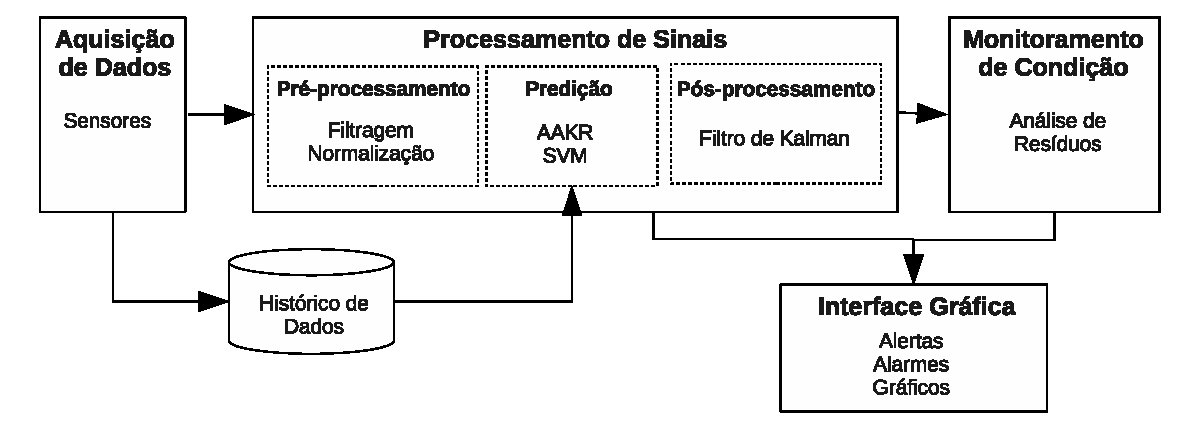
\includegraphics[width=\textwidth]{figuras/osa_cbm_drift.eps}
    % \end{figure}

    \note{
    \begin{itemize}
        \item Como se pode ver na figura, o kf pode vir como a etapa de pós-processamento,
            opcional, antes mesmo do SPRT
        \item Deixei-o para ser explicado depois porque seria necessário entender a
            utilidade dos resíduos
        \item suavidade: sem mudanças bruscas
    \end{itemize}}
    
\end{frame}

\begin{frame}{Sistemas Implementados}

    \begin{figure}[!htb]
        \centering Sistema 1
        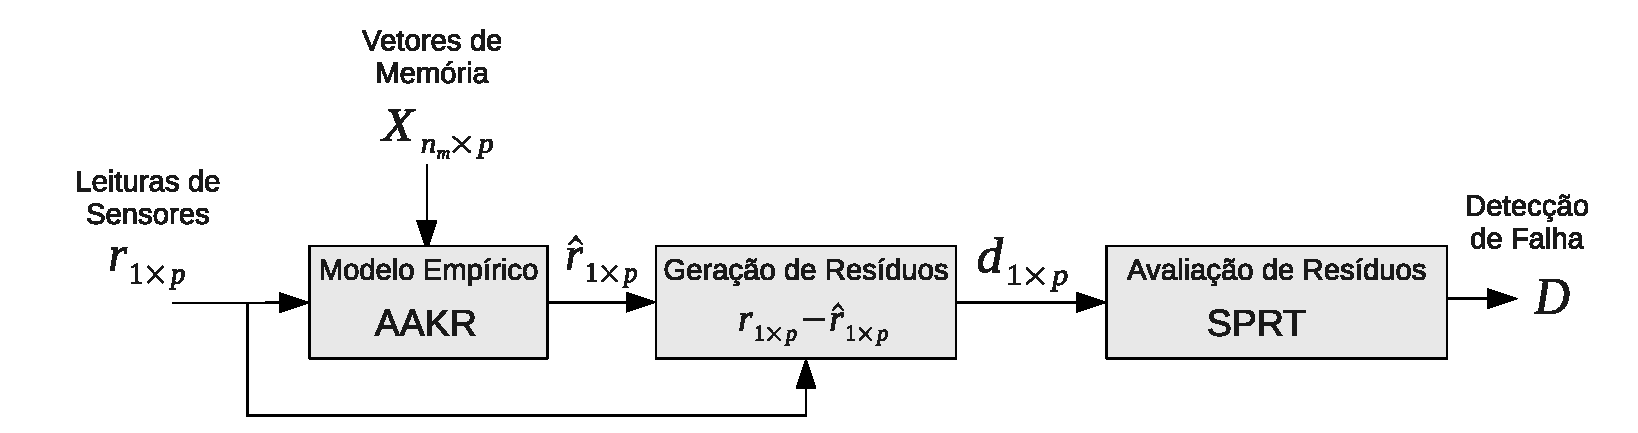
\includegraphics[width=.8\textwidth]{figuras/aakr_sprt.eps}
    \end{figure}
    
    \begin{figure}[!htb]
        \centering Sistema 2
        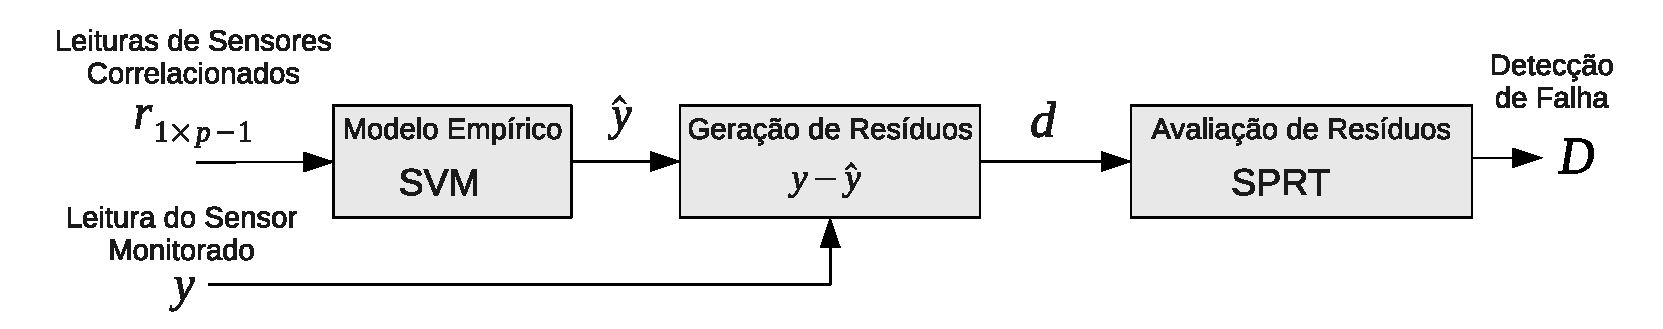
\includegraphics[width=.8\textwidth]{figuras/svm_sprt.eps}
    \end{figure}
    
    \begin{figure}[!htb]
        \centering Sistema 3
        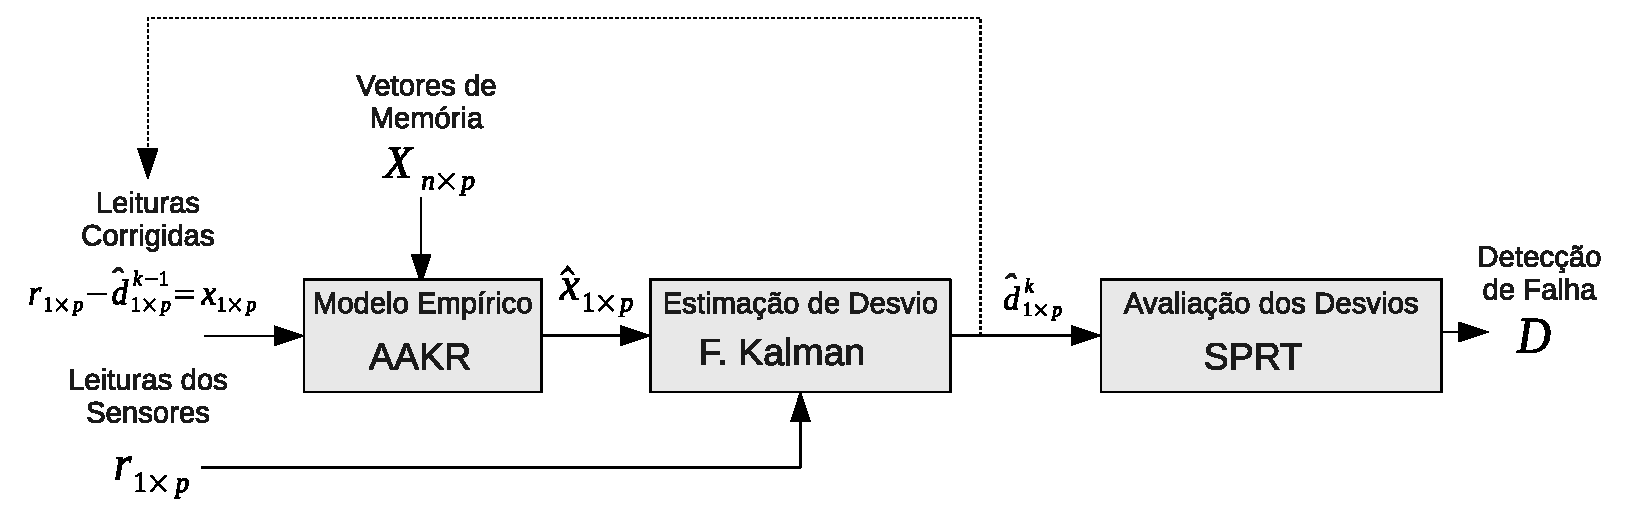
\includegraphics[width=.8\textwidth]{figuras/aakr_kf_sprt.eps}
    \end{figure}
    

    \note{
    \begin{itemize}
        \item 
    \end{itemize}}
    
\end{frame}


\section{Ensaios}

\begin{frame}{Análises dos Ensaios}

    \begin{itemize}
        \item Objetivo\\
            Verificar a \alert{aplicabilidade} dos sistemas a sensores de poços de petróleo
            \vspace{10pt}

        \item Critérios
            \begin{itemize}
                \item \alert{consistência} e \alert{qualidade} das predições
                \item capacidade de \alert{detecção} e \alert{isolamento} de desvios
            \end{itemize}
            \vspace{10pt}

        \item Como foram realizados\\
            Uso de conjuntos de dados compostos por amostras de diferentes
            \alert{sensores correlacionados}
            \begin{itemize}
                \item dados gerados por simulação
                \item dados reais
            \end{itemize}

    \end{itemize}

    \note{
    \begin{itemize}
        \item consistência e qualidade: considerando que se tem os valores ideais,
            verificar a proximidade das predições com esses valores
        \item detecção e isolamento: além de detectar a ocorrência de desvios, o sistema
            deve ser capaz de identificar o sensor falho
    \end{itemize}}
    
\end{frame}

\begin{frame}{Métricas de Desempenho}
    \begin{itemize}
        \item Acurácia ($E_a$)
            $$ E_a = \frac{1}{N} \sum \limits_{i=1}^N \left( \hat{r}^{(i)} - r^{(i)}
            \right)^2$$
        \item Erro de predição na ocorrência de desvios ($E_p$)
        \item Auto-sensibilidade ($S_A$) do sensor $p$
            $$
            S_{A_p} = \frac{1}{N} \sum \limits_{i=1}^N \frac{\left| \hat{r}_{p, drift}^{(i)} -
            \hat{r}^{(i)}_{p} \right|}{\left| r_{p,drift}^{(i)} - r^{(i)}_{p} \right|}
            $$
        \item Sensibilidade cruzada ($S_C$) do sensor $p$ em relação a $j$
            $$
            S_{C_{p,j}} = \frac{1}{N} \sum \limits_{i=1}^N \frac{\left| \hat{r}_{j,drift}^{(i)} -
            \hat{r}^{(i)}_{j} \right|}{\left| r_{p,drift}^{i} - r_{p}^{(i)} \right|}
            $$
    \end{itemize}

    \note{
    \begin{itemize}
        \item acurácia: mede a consistência e qualidade, a proximidade entre as predições
            e os valores verdadeiros, sem falhas
        \item erro de predição: semelhante à acurácia, medindo-se na presença de desvios,
            importante para medir a confiança nas predições na ocorrência de desvios
        \item auto-sensibilidade: sensibilidade do modelo a desvios no próprio sensor
        \item sensibilidade cruzada: sensibilidade do modelo para desvios em outros
            sensores
        \item as sensibilidades são calculadas inserindo desvios em um sensor por vez e,
            neste trabalho, tira-se a média dos sensores
    \end{itemize}}
    
\end{frame}

\subsection{Dados de Simulação}

\begin{frame}{Descrição dos Dados de Simulação}
    
    \begin{columns}[T]
        \column{.35\textwidth}
        \begin{figure}[!htb]
            \centering
            \includegraphics[height=.8\textheight]{figuras/poco_simulado.ps}
        \end{figure}
        \column{.55\textwidth}
        Modelo próximo de um poço real
        \begin{itemize}
            \item 4 sensores de pressão:
                \begin{itemize}
                    \item fundo do poço (PT$_f$)
                    \item topo do tubo de produção (PT$_t$)
                    \item topo do anular (PT$_g$)
                    \item a montante do \textit{choke} de injeção (PT$_m$)
                \end{itemize}
            \item Coletado durante 100 horas de produção
            \item Amostrado em 1 minuto
            \item Ruído branco de NSR (\textit{noise to signal ratio}) igual a 0.3
            \item 60 horas como treinamento, 20 de otimização e 20 de teste
        \end{itemize}
    \end{columns}

\end{frame}

\begin{frame}{Gráficos dos Dados de Simulação}

    \begin{figure}[!htb]
        \centering
        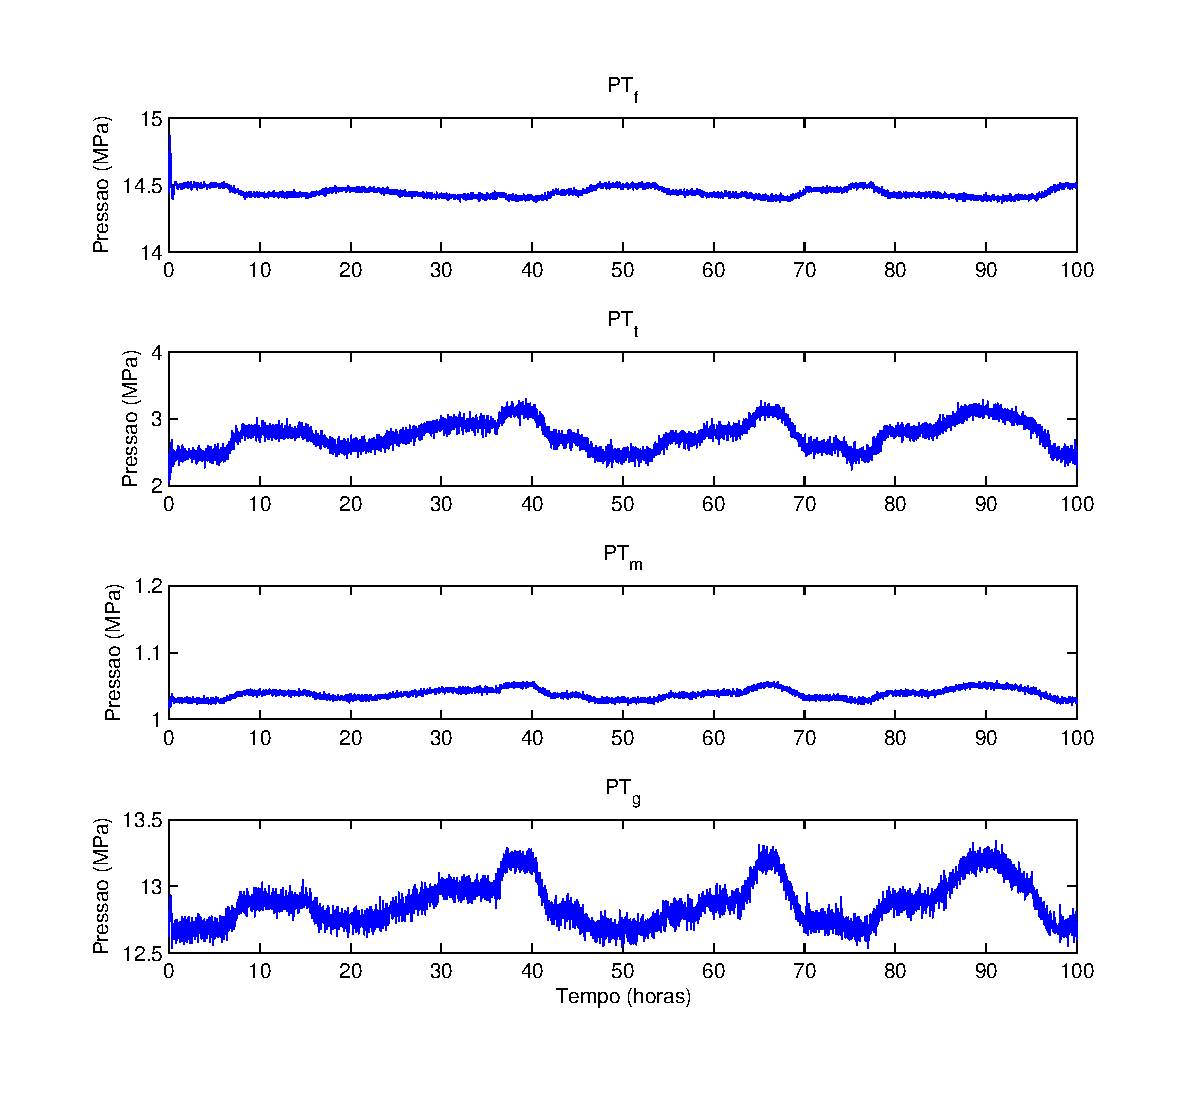
\includegraphics[height=\textheight]{figuras/sim_dataset.eps}
    \end{figure}

    \note{
    Mostrar divisão dos conjuntos de treinamento, otimização e teste}
    
\end{frame}

\begin{frame}{Indicadores de Desempenho\\Dados de Simulação}

    \begin{table}[bt]
        \centering
    \begin{tabular}{lcccc}
        \toprule
        & $E_a$ & $S_A$ & $S_C$ & $E_p$ \\
        \midrule
        Sistema 1 & 0.0020 & 0.2675 & 0.2682 & 0.0105 \\
        Sistema 2 & 0.0039 & & 0.3356 & 0.0139 \\
        Sistema 3 & 0.0023 & 0.2002 & 0.1997 & 0.0046 \\
        \bottomrule
    \end{tabular}
    \end{table}

    \note{
    \begin{itemize}
        \item valor nulo de $S_A$: os modelos SVM estimam dados de um sensor que não é
            usado como input (inferencial)
    \end{itemize}}

\end{frame}

\begin{frame}{Predições para Desvios em PT$_g$}

    \begin{itemize}
        \item \color{red}{Predições} 
        \item \color{green}{Entradas} 
        \item \color{blue}{Verdadeiro}
    \end{itemize}
    \vspace*{-15pt}
    \begin{figure}[bt]
        \centering\hspace*{-20pt}
        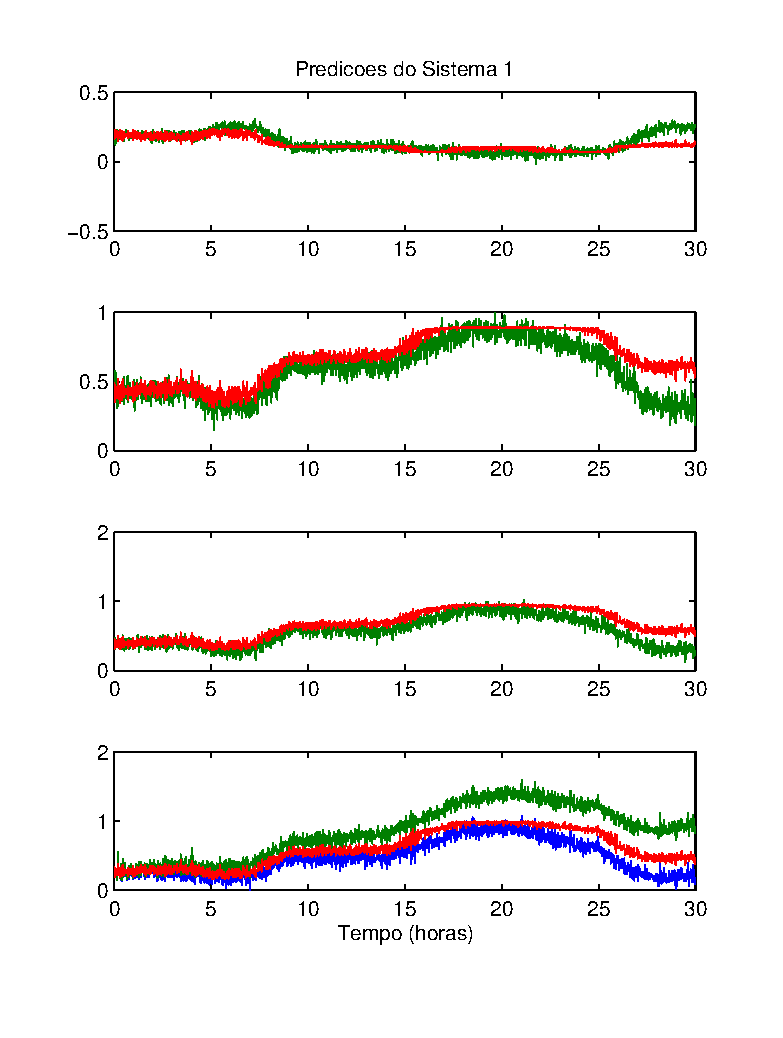
\includegraphics[trim=1cm .7cm 1cm .5cm, clip=true,width=.37\textwidth]{figuras/sim_sys1_pred_d4.eps}
        \includegraphics[trim=1cm .7cm 1cm .5cm, clip=true,width=.37\textwidth]{figuras/sim_sys2_pred_d4.eps}
        \includegraphics[trim=1cm .7cm 1cm .5cm, clip=true,width=.37\textwidth]{figuras/sim_sys3_pred_d4.eps}
    \end{figure}

    \note{
    \begin{itemize}
        \item sistema 1: predições pioram a medida que os desvios se acentuam, a ponto de
            não conseguir gerar predições por não haver vetores de memória similares nos
            dados de treinamento
        \item sistema 2: as predições que dependem do sensor PT$_g$ ficam muito degradadas
            com o crescimento dos desvios; o modelo corresponde a uma função e pra vetores
            de dados muito diferentes dos dados de treino as predições ficam imprevisíveis
        \item sistema 3: estimando os desvios, consegue-se uma certa correção das
            predições, mantendo um desempenho mais constante mesmo para desvios grandes,
            apesar do bias
    \end{itemize}}

\end{frame}

\begin{frame}{Detecção de Desvios nos Dados de Simulação\\Sistema 1}
    
    \begin{figure}[bt]
        \centering\hspace*{-15pt}
        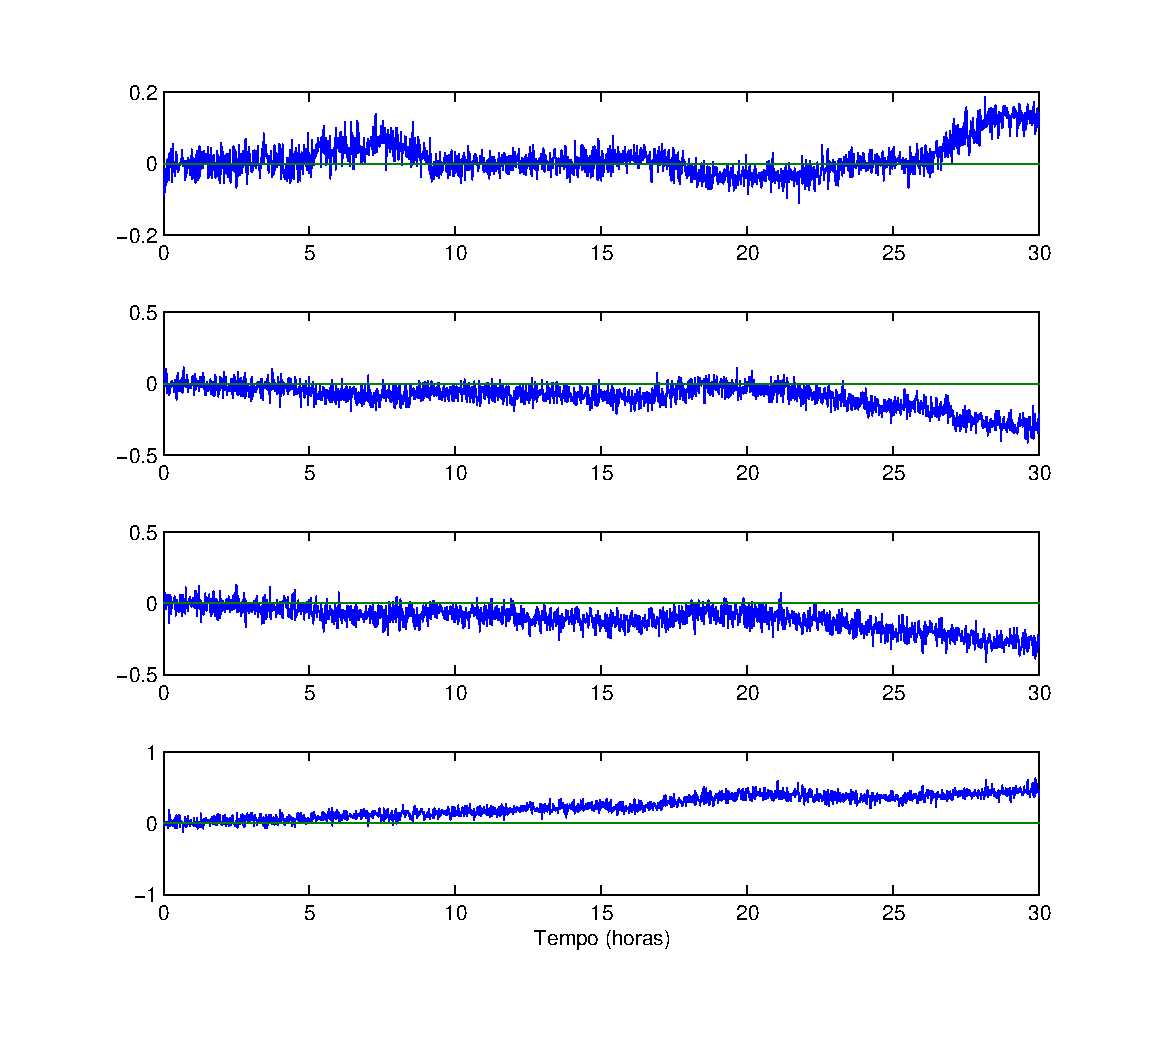
\includegraphics[trim=1.5cm .7cm 1.1cm .7cm,clip=true,width=.55\textwidth]{figuras/sim_sys1_resid_d4.eps}
        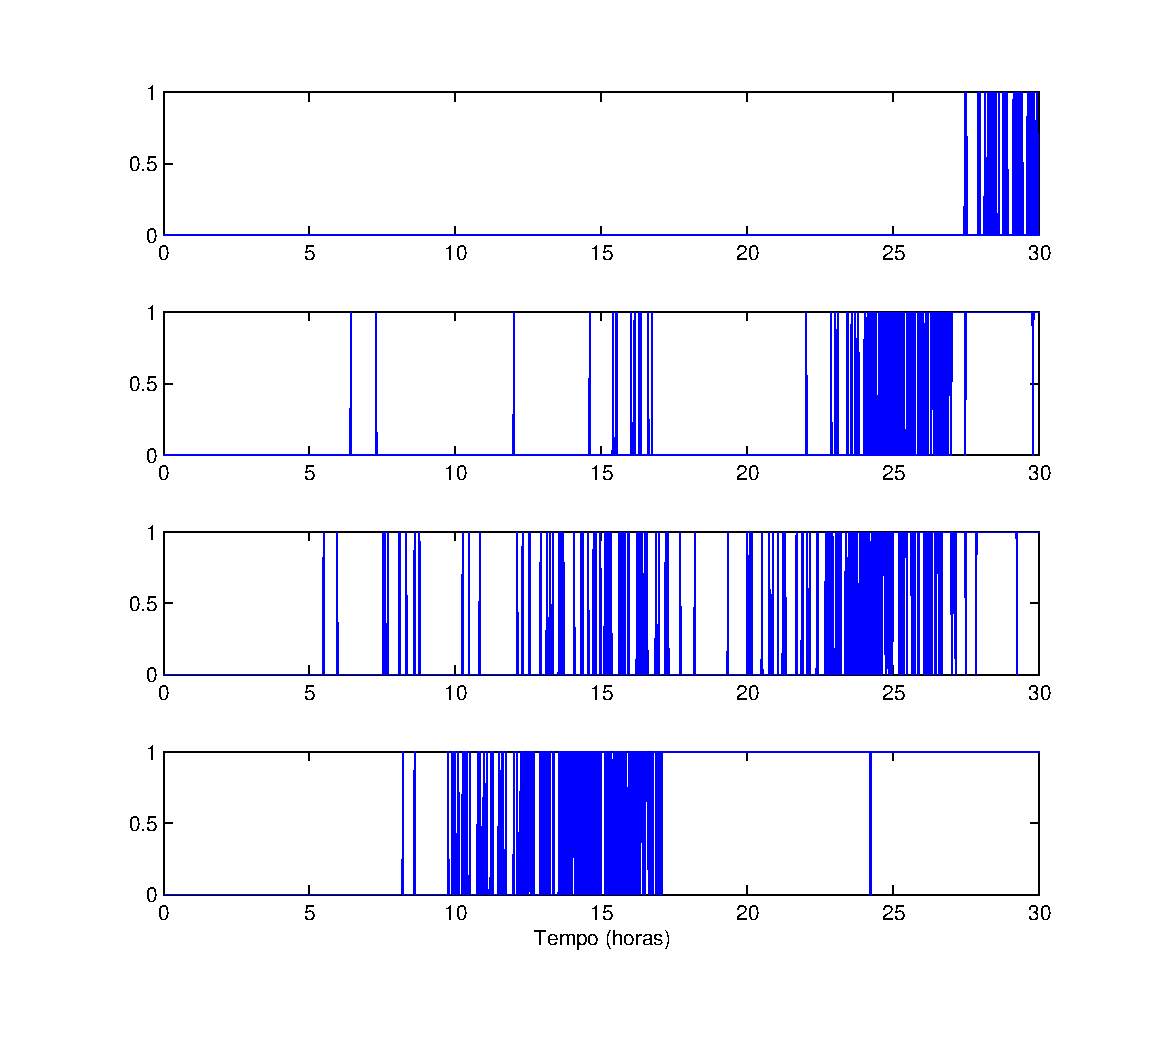
\includegraphics[trim=1.5cm .7cm 1.1cm .7cm,clip=true,width=.55\textwidth]{figuras/sim_sys1_sprt_d4.eps}
    \end{figure}

    \note{
    \begin{itemize}
        \item O ideal é que se consiga detectar os desvios antes que as predições fiquem
            muito degradadas
        \item apesar dos falsos alarmes para PT$_m$, se víssemos mais de perto as
            decisões, perceberíamos que ocorrem poucos falsos alarmes consecutivos
        \item alarmes verdadeiros ocorrem de forma consecutiva
        \item outra forma de melhor o isolamento é ajustar melhor o valor de $M$, com a
            possibilidade de uma detecção mais tardia
    \end{itemize}}
\end{frame}

\begin{frame}{Detecção de Desvios nos Dados de Simulação\\Sistema 2}

    \begin{figure}[bt]
        \centering\hspace*{-15pt}
        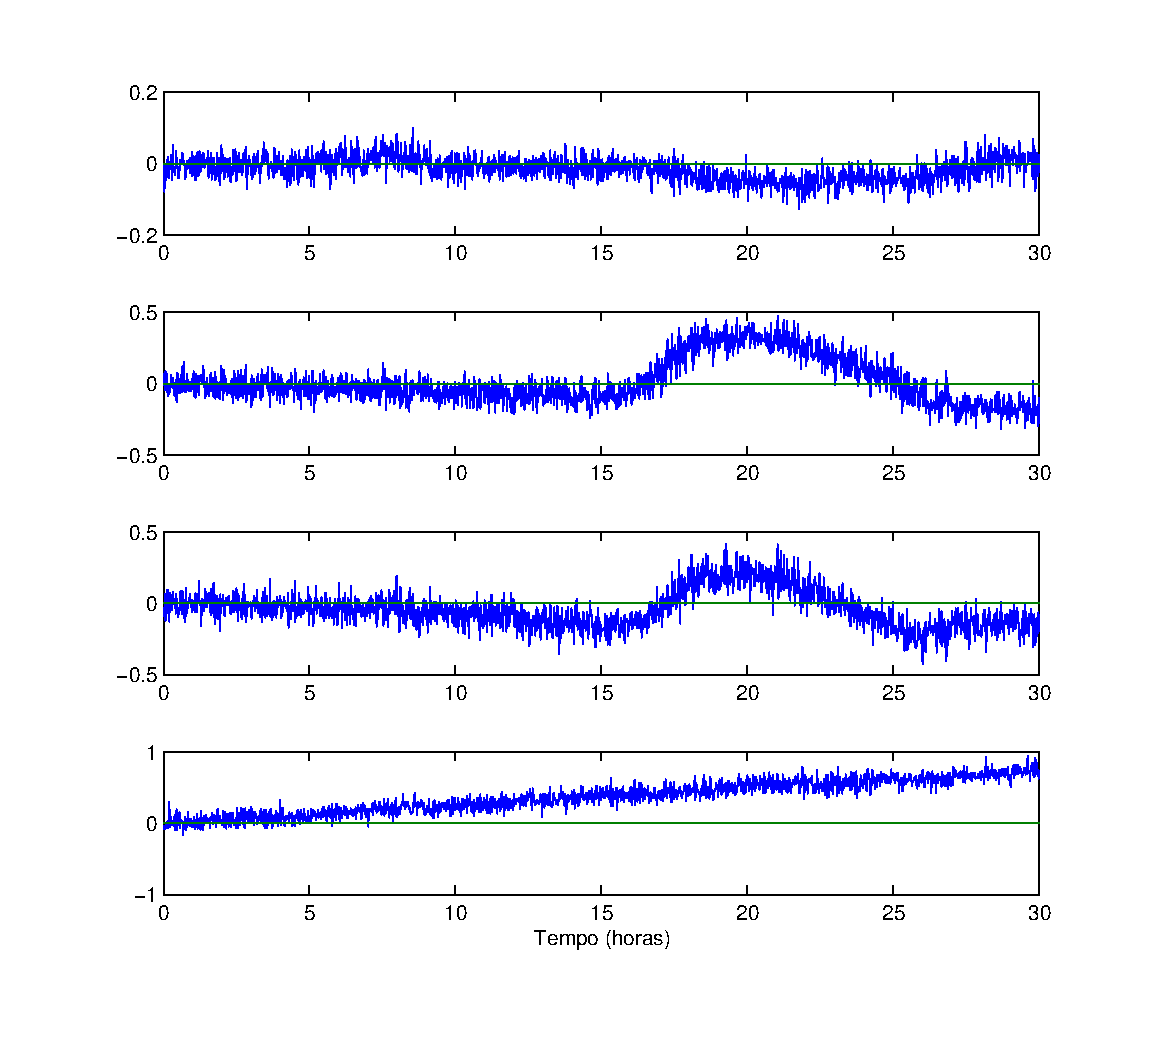
\includegraphics[trim=1.5cm .7cm 1.1cm .7cm,clip=true,width=.55\textwidth]{figuras/sim_svm_resid_d4.eps}
        \includegraphics[trim=1.5cm .7cm 1.1cm .7cm,clip=true,width=.55\textwidth]{figuras/sim_svm_sprt_d4.eps}
    \end{figure}

    \note{
    \begin{itemize}
        \item apesar das piores predições na ocorrência de desvios severos, a detecção e
            isolamento dos desvios é bem clara, devido à boa predição de PT$_g$
        \item funciona bem para a detecção de desvios, mas se pode confiar muito nas
            predições quando uma ocorrência é detectada
    \end{itemize}}
\end{frame}

\begin{frame}{Detecção de Desvios nos Dados de Simulação\\Sistema 3}

    \begin{figure}[bt]
        \centering\hspace*{-15pt}
        \includegraphics[trim=1.5cm .7cm 1.1cm .7cm,clip=true,width=.55\textwidth]{figuras/sim_sys3_resid_d4.eps}
        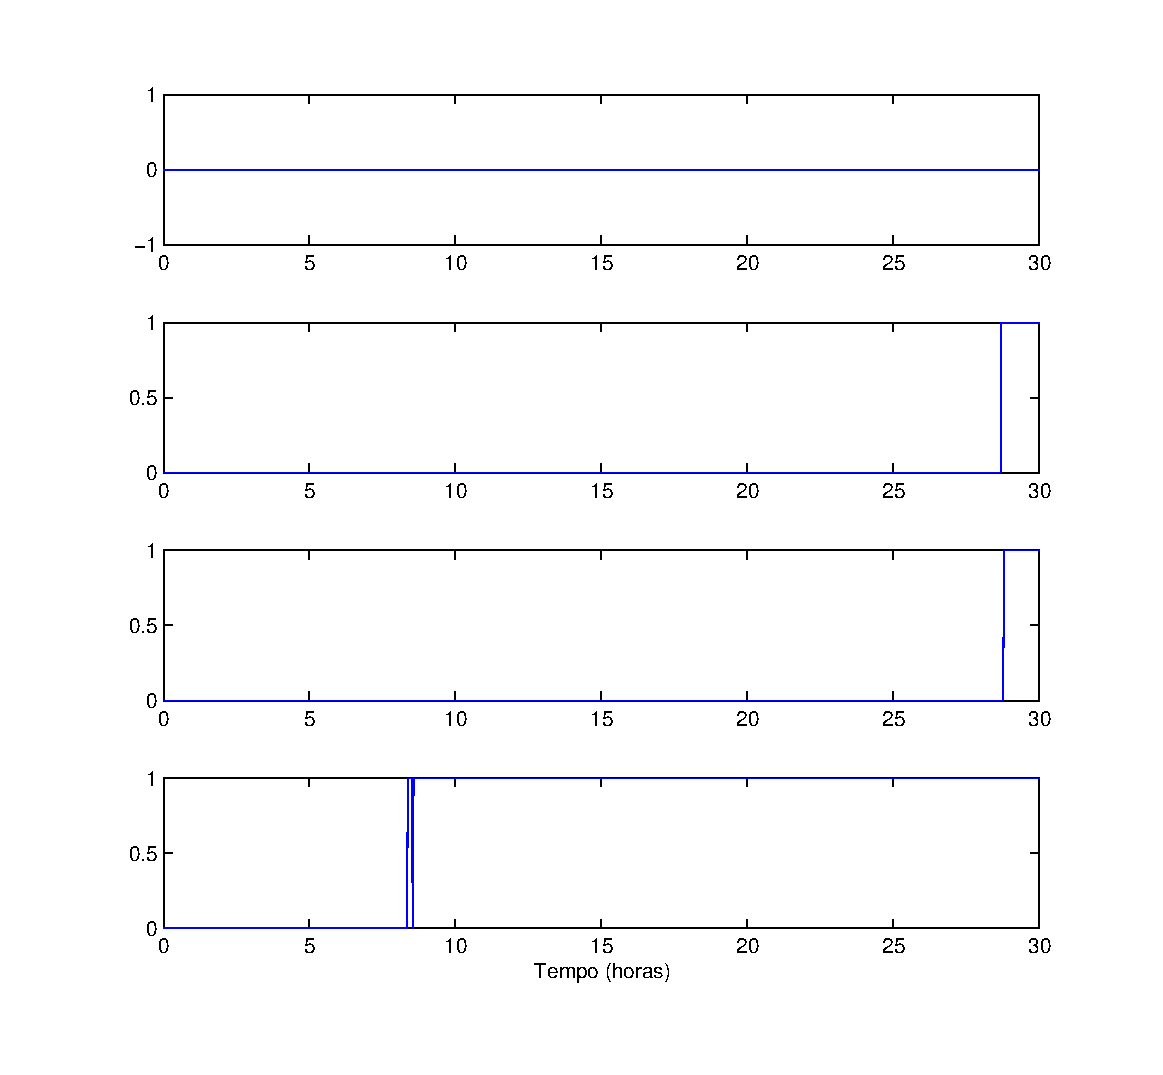
\includegraphics[trim=1.5cm .7cm 1.1cm .7cm,clip=true,width=.55\textwidth]{figuras/sim_sys3_sprt_d4.eps}
    \end{figure}

    \note{
    \begin{itemize}
        \item neste caso, usam-se as estimativas do filtro de kalman para a detecção e
            isolamento
        \item nota-se a diferença entre as estimativas pela escala do gráfico; ficaria
            melhor se estivessem na mesma escala
        \item falsos alarmes ocorrem apenas quando os desvios estão grandes
        \item então, o sistema 3 também corresponde aos critérios aplicabilidade
    \end{itemize}}
\end{frame}

\subsection{Dados Reais}

\begin{frame}{Descrição dos Dados Reais}
    
    \begin{itemize}
        \item Pressão coletada de 3 sensores
            \begin{itemize}
                \item no fundo do poço (PDG)
                \item na árvore de natal (TPT)
                \item a montante do choke de injeção (PT$_m$)
            \end{itemize}
        \item Coletados durante 955 horas de produção
            \begin{itemize}
                \item 400 primeiras horas para treinamento
                \item 100 para otimização
                \item 455 para teste
            \end{itemize}
        \item Amostragem de 1 por minuto
    \end{itemize}
\end{frame}

\begin{frame}{Gráficos dos Dados Reais}

\begin{figure}[bt]
    \centering
    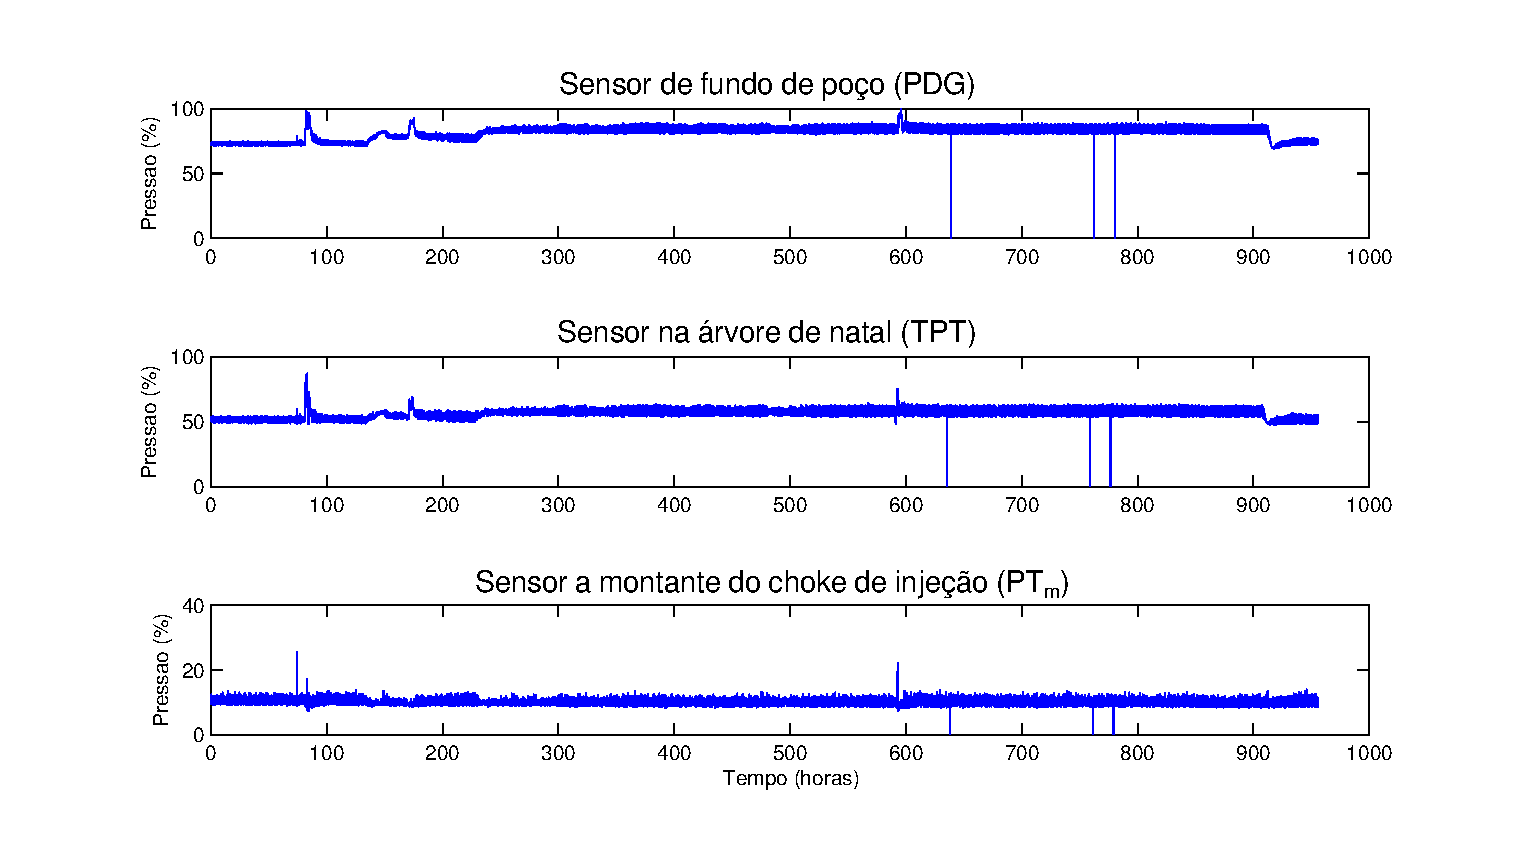
\includegraphics[trim=2cm .7cm 2cm .7cm,clip=true,width=\textwidth]{figuras/real_dataset.eps}
\end{figure}

\note{
\begin{itemize}
    \item gráficos escalados para 0-100\%
    \item outliers (dados faltantes) estão representados como $-1$
\end{itemize}}
    
\end{frame}

\begin{frame}{Indicadores de Desempenho\\Dados Reais}

\begin{table}[bt]
    \centering
    \begin{tabular}{lcccc}
        \toprule
        & $E_a$ & $S_A$ & $S_C$ & $E_p$ \\
        \midrule
        Sistema 1 & 0.0035 & 0.3106 & 0.2806 & 0.0078 \\
        Sistema 2 & 0.0069 &  & 0.4754 & 0.0190 \\
        Sistema 3 & 0.0040 & 0.2418 & 0.2189 & 0.0046 \\
        \bottomrule
    \end{tabular}
\end{table}
\end{frame}

\begin{frame}{Predições para Desvios no PDG}
    
    \begin{itemize}
        \item \color{red}{Predições} 
        \item \color{green}{Entradas} 
        \item \color{blue}{Verdadeiro}
    \end{itemize}
    \vspace*{-20pt}

    \begin{figure}[bt]
        \centering\hspace*{-20pt}
        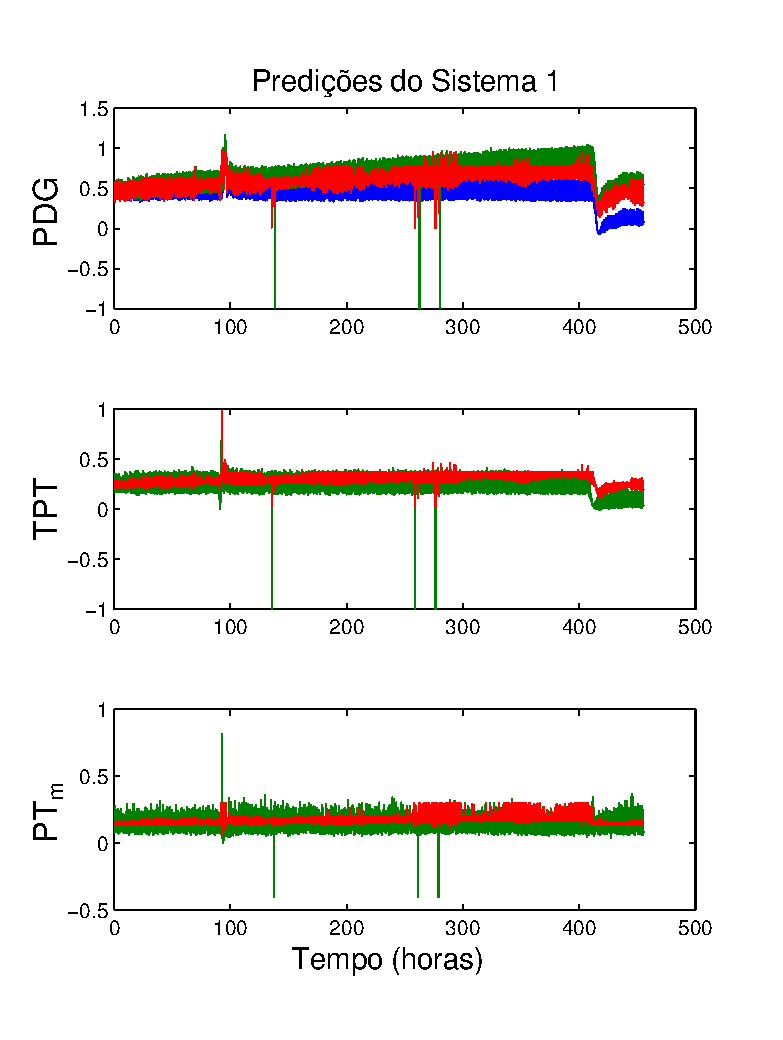
\includegraphics[trim=1cm .7cm .8cm .1cm, clip=true,width=.37\textwidth]{figuras/real_aakr_pred_d1.eps}
        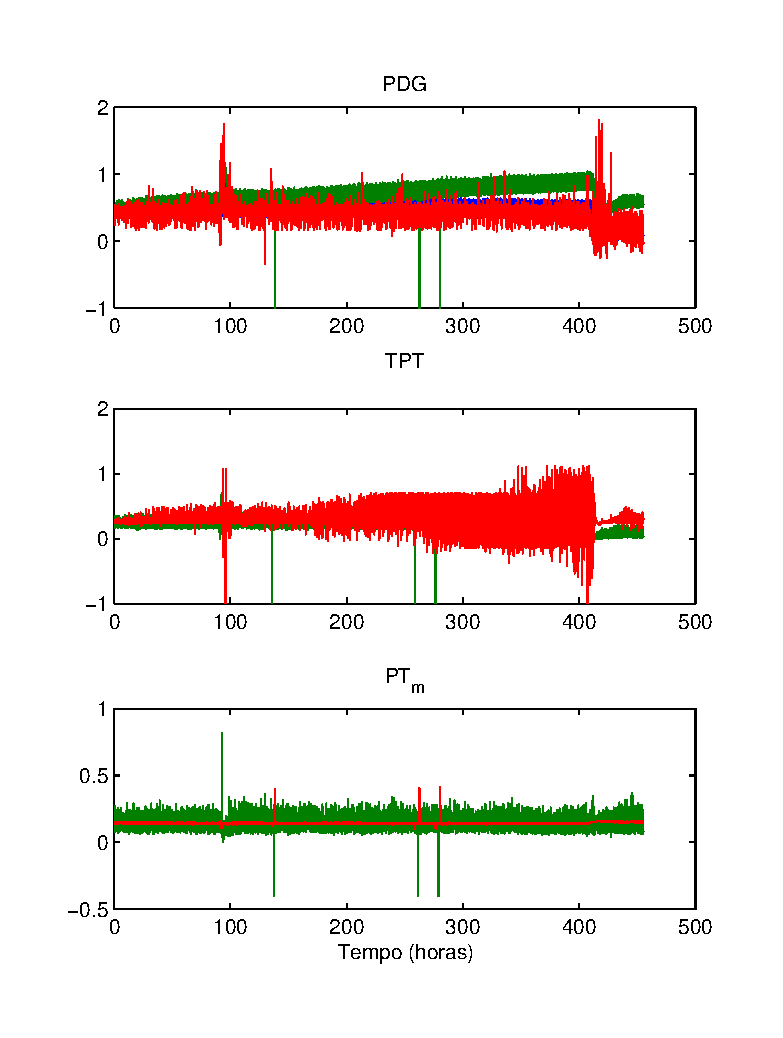
\includegraphics[trim=1cm .7cm .8cm .1cm, clip=true,width=.37\textwidth]{figuras/real_svm_pred_d1.eps}
        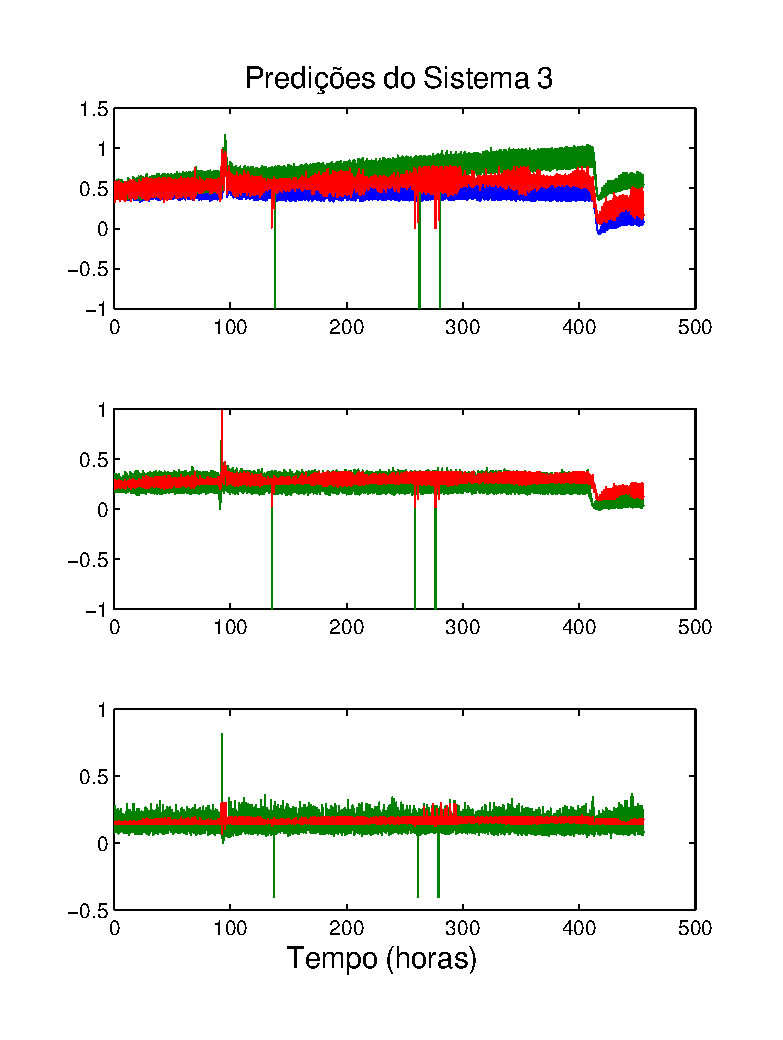
\includegraphics[trim=1cm .7cm .8cm .1cm, clip=true,width=.37\textwidth]{figuras/real_aakr_kf_pred_d1.eps}
    \end{figure}

    \note{
    \begin{itemize}
        \item Problemas no sistema 2: pouca informação, ruídos e desvios
    \end{itemize}}
\end{frame}

\begin{frame}{Detecção de Desvios nos Dados Reais\\Sistema 1}
    
    \begin{figure}[bt]
        \centering\hspace*{-15pt}
        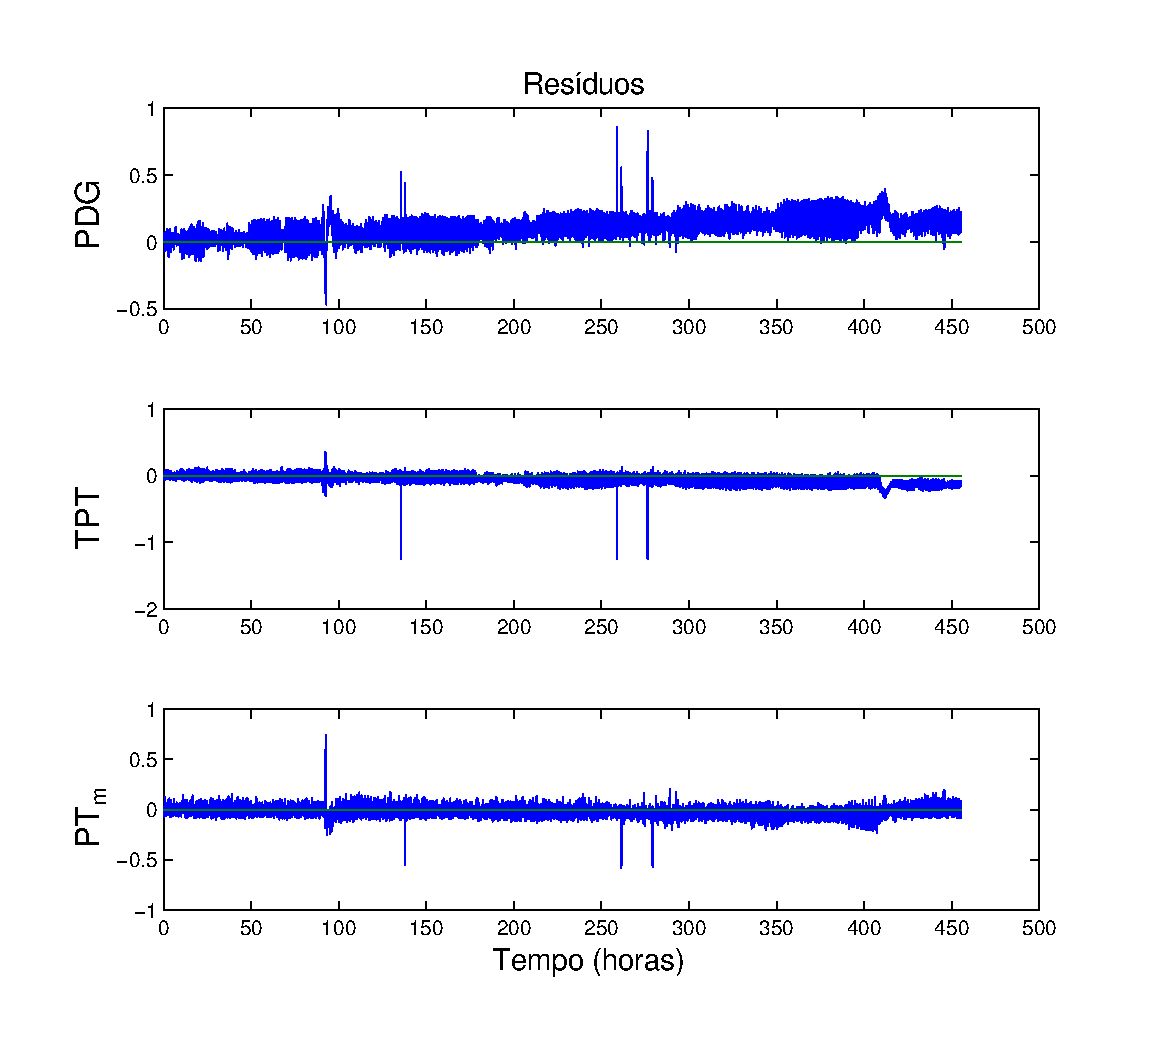
\includegraphics[trim=1.5cm .7cm 1.1cm .7cm,clip=true,width=.55\textwidth]{figuras/real_sys1_res_d1.eps}
        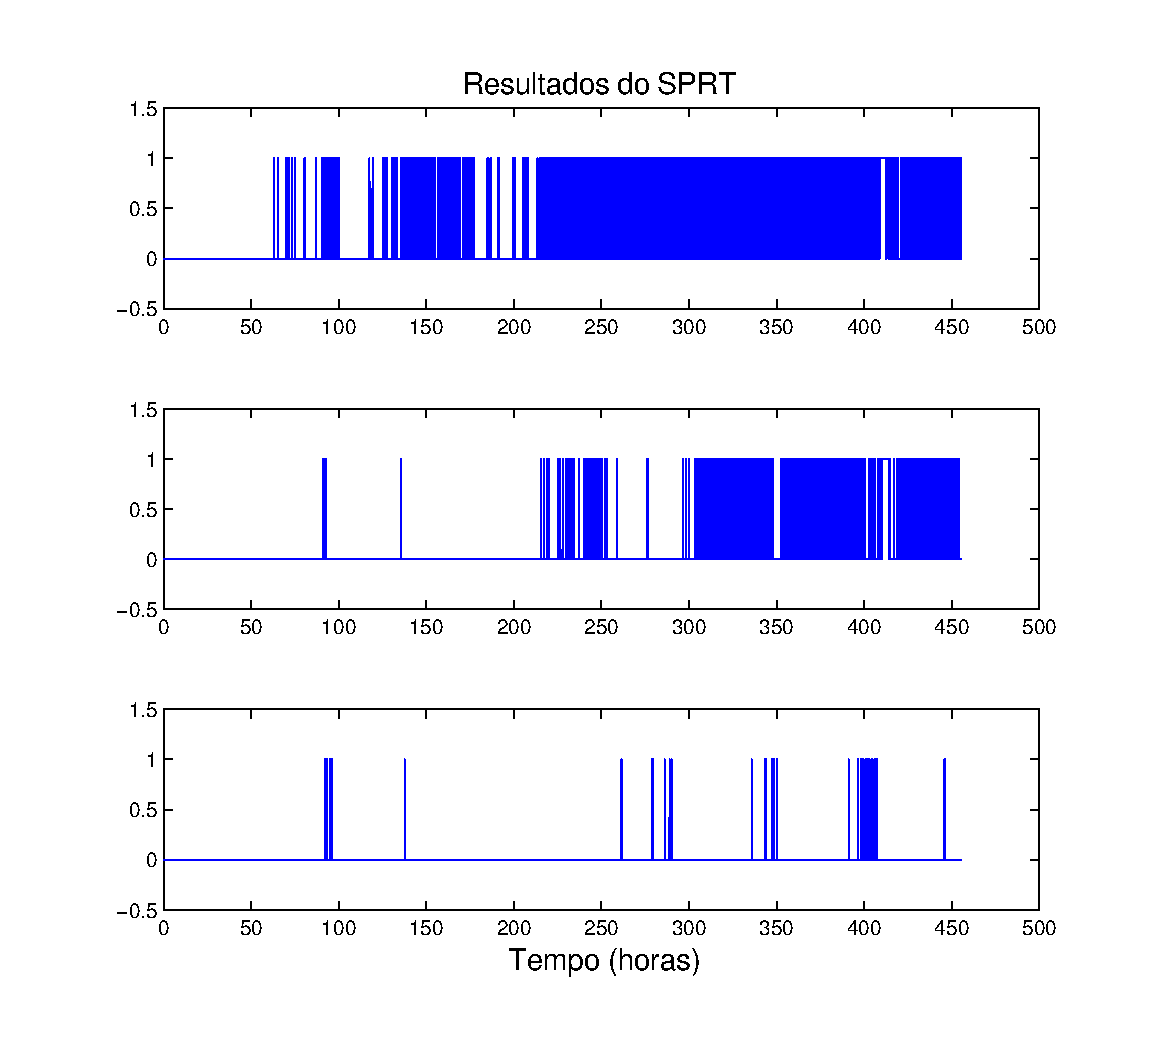
\includegraphics[trim=1.5cm .7cm 1.1cm .7cm,clip=true,width=.55\textwidth]{figuras/real_sys1_sprt_d1.eps}
    \end{figure}
\end{frame}

\begin{frame}{Detecção de Desvios nos Dados Reais\\Sistema 2}
    \begin{figure}[bt]
        \centering\hspace*{-15pt}
        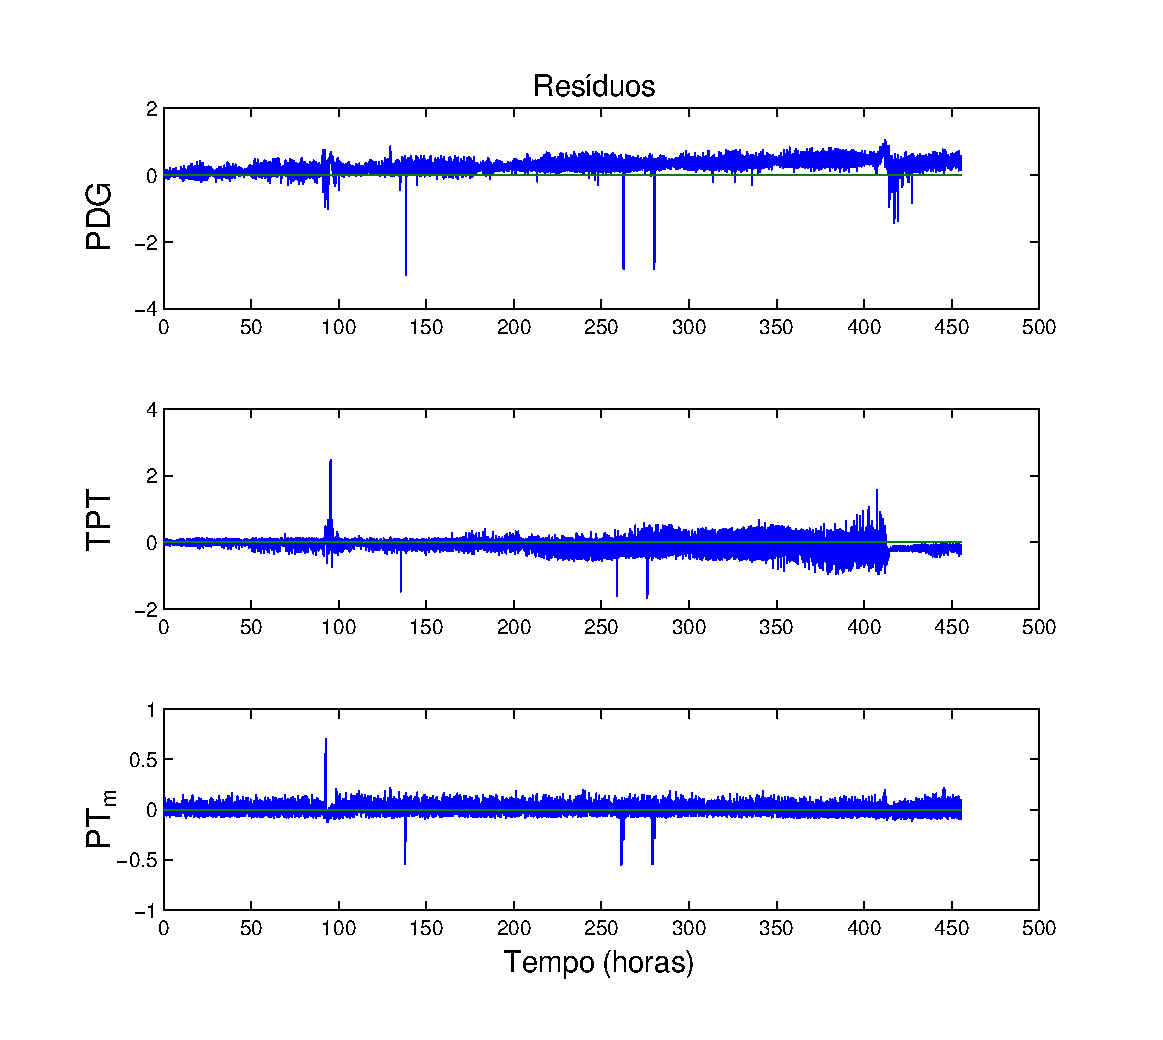
\includegraphics[trim=1.5cm .7cm 1.1cm .7cm,clip=true,width=.55\textwidth]{figuras/real_sys2_res_d1.eps}
        \includegraphics[trim=1.5cm .7cm 1.1cm .7cm,clip=true,width=.55\textwidth]{figuras/real_sys2_sprt_d1.eps}
    \end{figure}
\end{frame}

\begin{frame}{Detecção de Desvios nos Dados Reais\\Sistema 3}
    \begin{figure}[bt]
        \centering\hspace*{-15pt}
        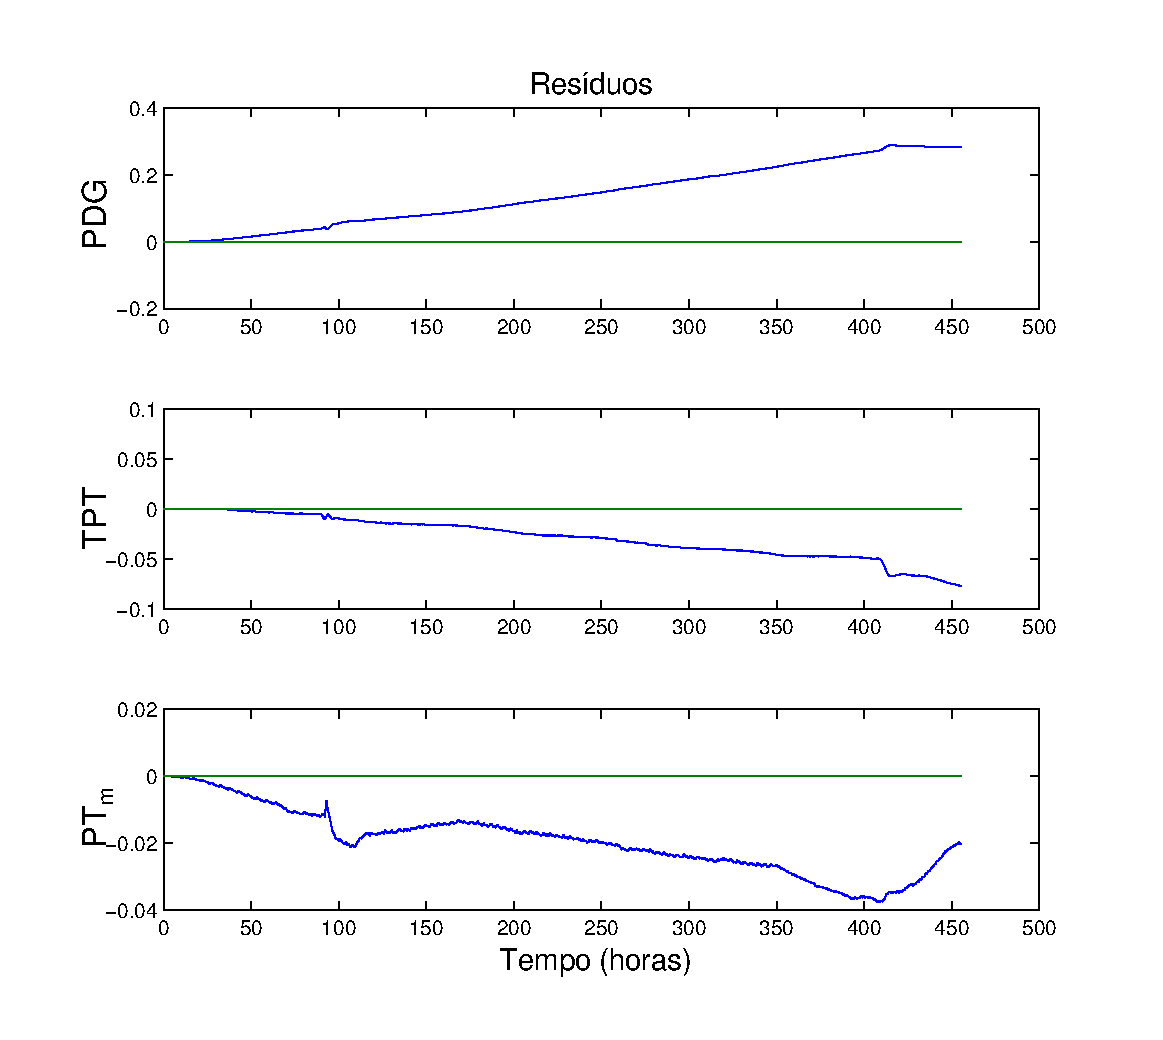
\includegraphics[trim=1.5cm .7cm 1.1cm .7cm,clip=true,width=.55\textwidth]{figuras/real_sys3_res_d1.eps}
        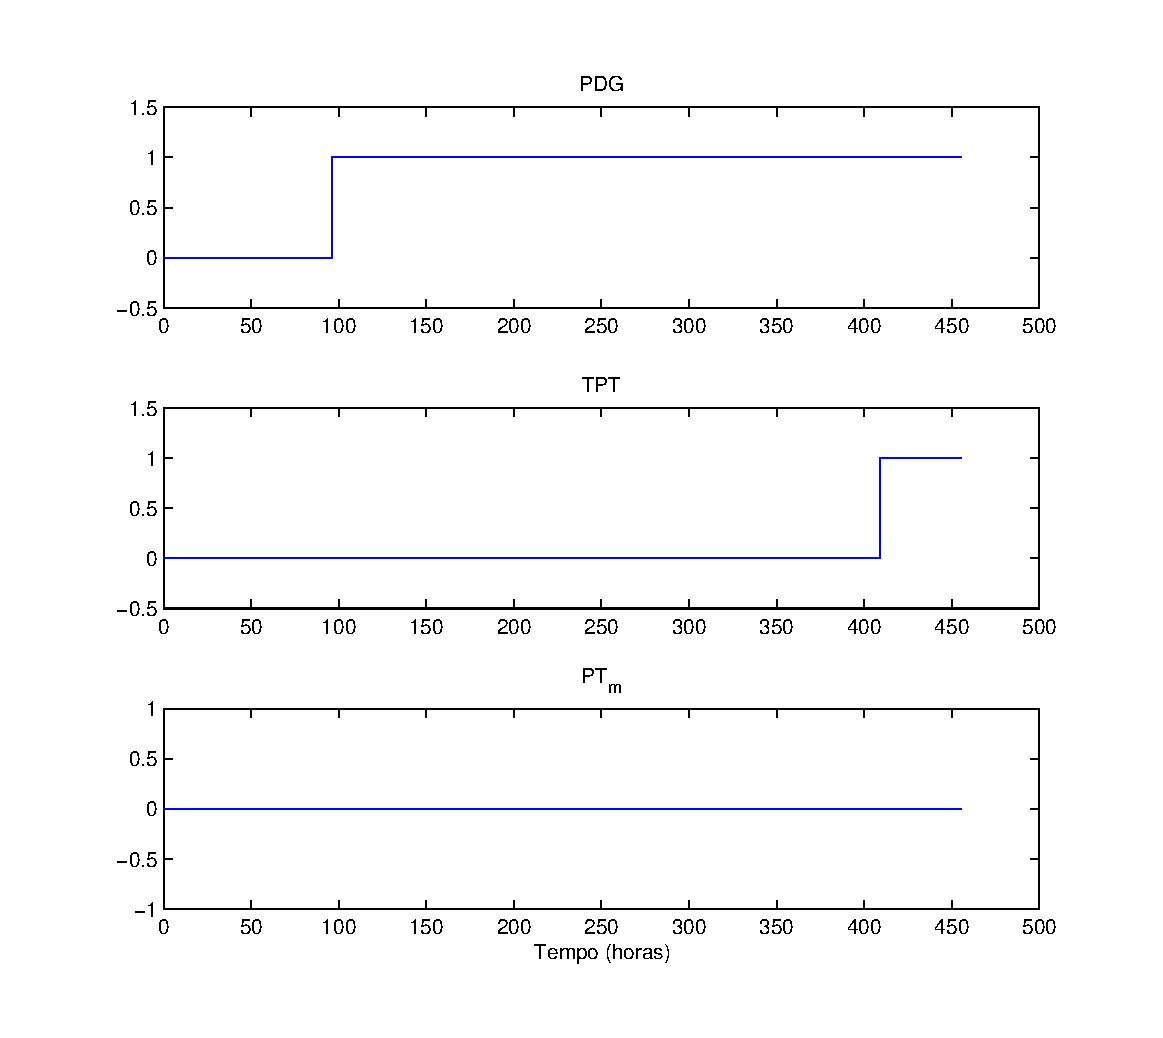
\includegraphics[trim=1.5cm .7cm 1.1cm .7cm,clip=true,width=.55\textwidth]{figuras/real_sys3_sprt_d1.eps}
    \end{figure}
\end{frame}

\section{Conclusão}
\subsection{}

\begin{frame}{Conclusões}

    \begin{itemize}
        \item Importância dos sensores na indústria de petróleo
        \item Problemas de \textit{drifts} ou desvios
        \item Proposta do trabalho
        \item Implementação de 3 diferentes sistemas de detecção de desvios
            \begin{itemize}
                \item Sistema 1: AAKR e SPRT
                \item Sistema 2: SVM e SPRT
                \item Sistema 3: AAKR, KF e SPRT
            \end{itemize}
        \item Ensaios
            \begin{itemize}
                \item simulação\\
                    todos os sistemas detectaram desvios corretamente
                \item dados reais\\
                    o Sistema 2 apresentou problemas
                \item KF tem uso promissor
            \end{itemize}
    \end{itemize}

    \note{
    \begin{itemize}
        \item importância dos sensores: ações de controle, otimização da produção e tomada
            de decisões
        \item problemas do sistema 2 nos dados reais: apesar dos problemas, não seria uma
            boa ideia descartar o emprego de modelos SVM, uma vez que tratamentos mais
            adequados ou casos com mais sensores envolvidos podem gerar bons resultados
    \end{itemize}}
    
\end{frame}

\begin{frame}{Conclusões}
    
    Problemas com a abordagem por modelos baseados em histórico:
    \begin{itemize}
        \item Agrupamento ótimo de sensores
        \item Seleção dos dados de treinamento
            \begin{itemize}
                \item livres de falhas
                \item cobertura das condições de operação futuras
            \end{itemize}
        \item Discernir entre mudanças no processo e falhas nos sensores
    \end{itemize}
    
\end{frame}

\begin{frame}{Trabalhos Futuros}
    \begin{itemize}
        \item Agrupamento automático de sensores
        \item Validação dos modelos empíricos
        \item Modelos SVM para predição de séries temporais
    \end{itemize}

    \note{
    \begin{itemize}
        \item agrupamento: tećnicas para agrupamento ótimo, com grupos mais
            correlacionados
        \item validação dos modelos: características do poço mudam com tempo; analisar
            formas de discernir entre falhas em sensores e mudanças no poço
        \item modelos SVM: considerar na modelagem a dependência entre as amostras de
            instantes consecutivos, dinâmica
    \end{itemize}}
\end{frame}

\begin{frame}
    \titlepage
    
\end{frame}

\end{document}
